% "{'classe':('PSI','PT'),'chapitre':'oral_mt','type':('oral_mt'),'titre':'Réplique de la mission InSIGHT', 'source':'Concours Commun INP 2019 MP','comp':(),'corrige':False}"
%\setchapterimage{bandeau}
\chapter*{Préparation Mines Telecom \\%\arabic{cptColle} \\ 
Réplique de la mission InSIGHT \ifnormal $\star$ \else \fi \iftdifficile $\star\star\star$ \else \fi  -- 
\ifprof Corrigé \else Sujet \fi}
\addcontentsline{toc}{section}{Colle \arabic{cptColle} :
Réplique de la mission InSIGHT \ifnormal $\star$ \else \fi \iftdifficile $\star\star\star$ \else \fi  -- 
\ifprof Corrigé \else Sujet \fi}

\iflivret \stepcounter{cptColle} \else
\ifprof  \stepcounter{cptColle} \else \fi
\fi

\setcounter{question}{0}
\marginnote{D'après concours Commun INP 2019 -- MP.}
\marginnote{
\UPSTIcompetence[2]{}
}


\begin{marginfigure}
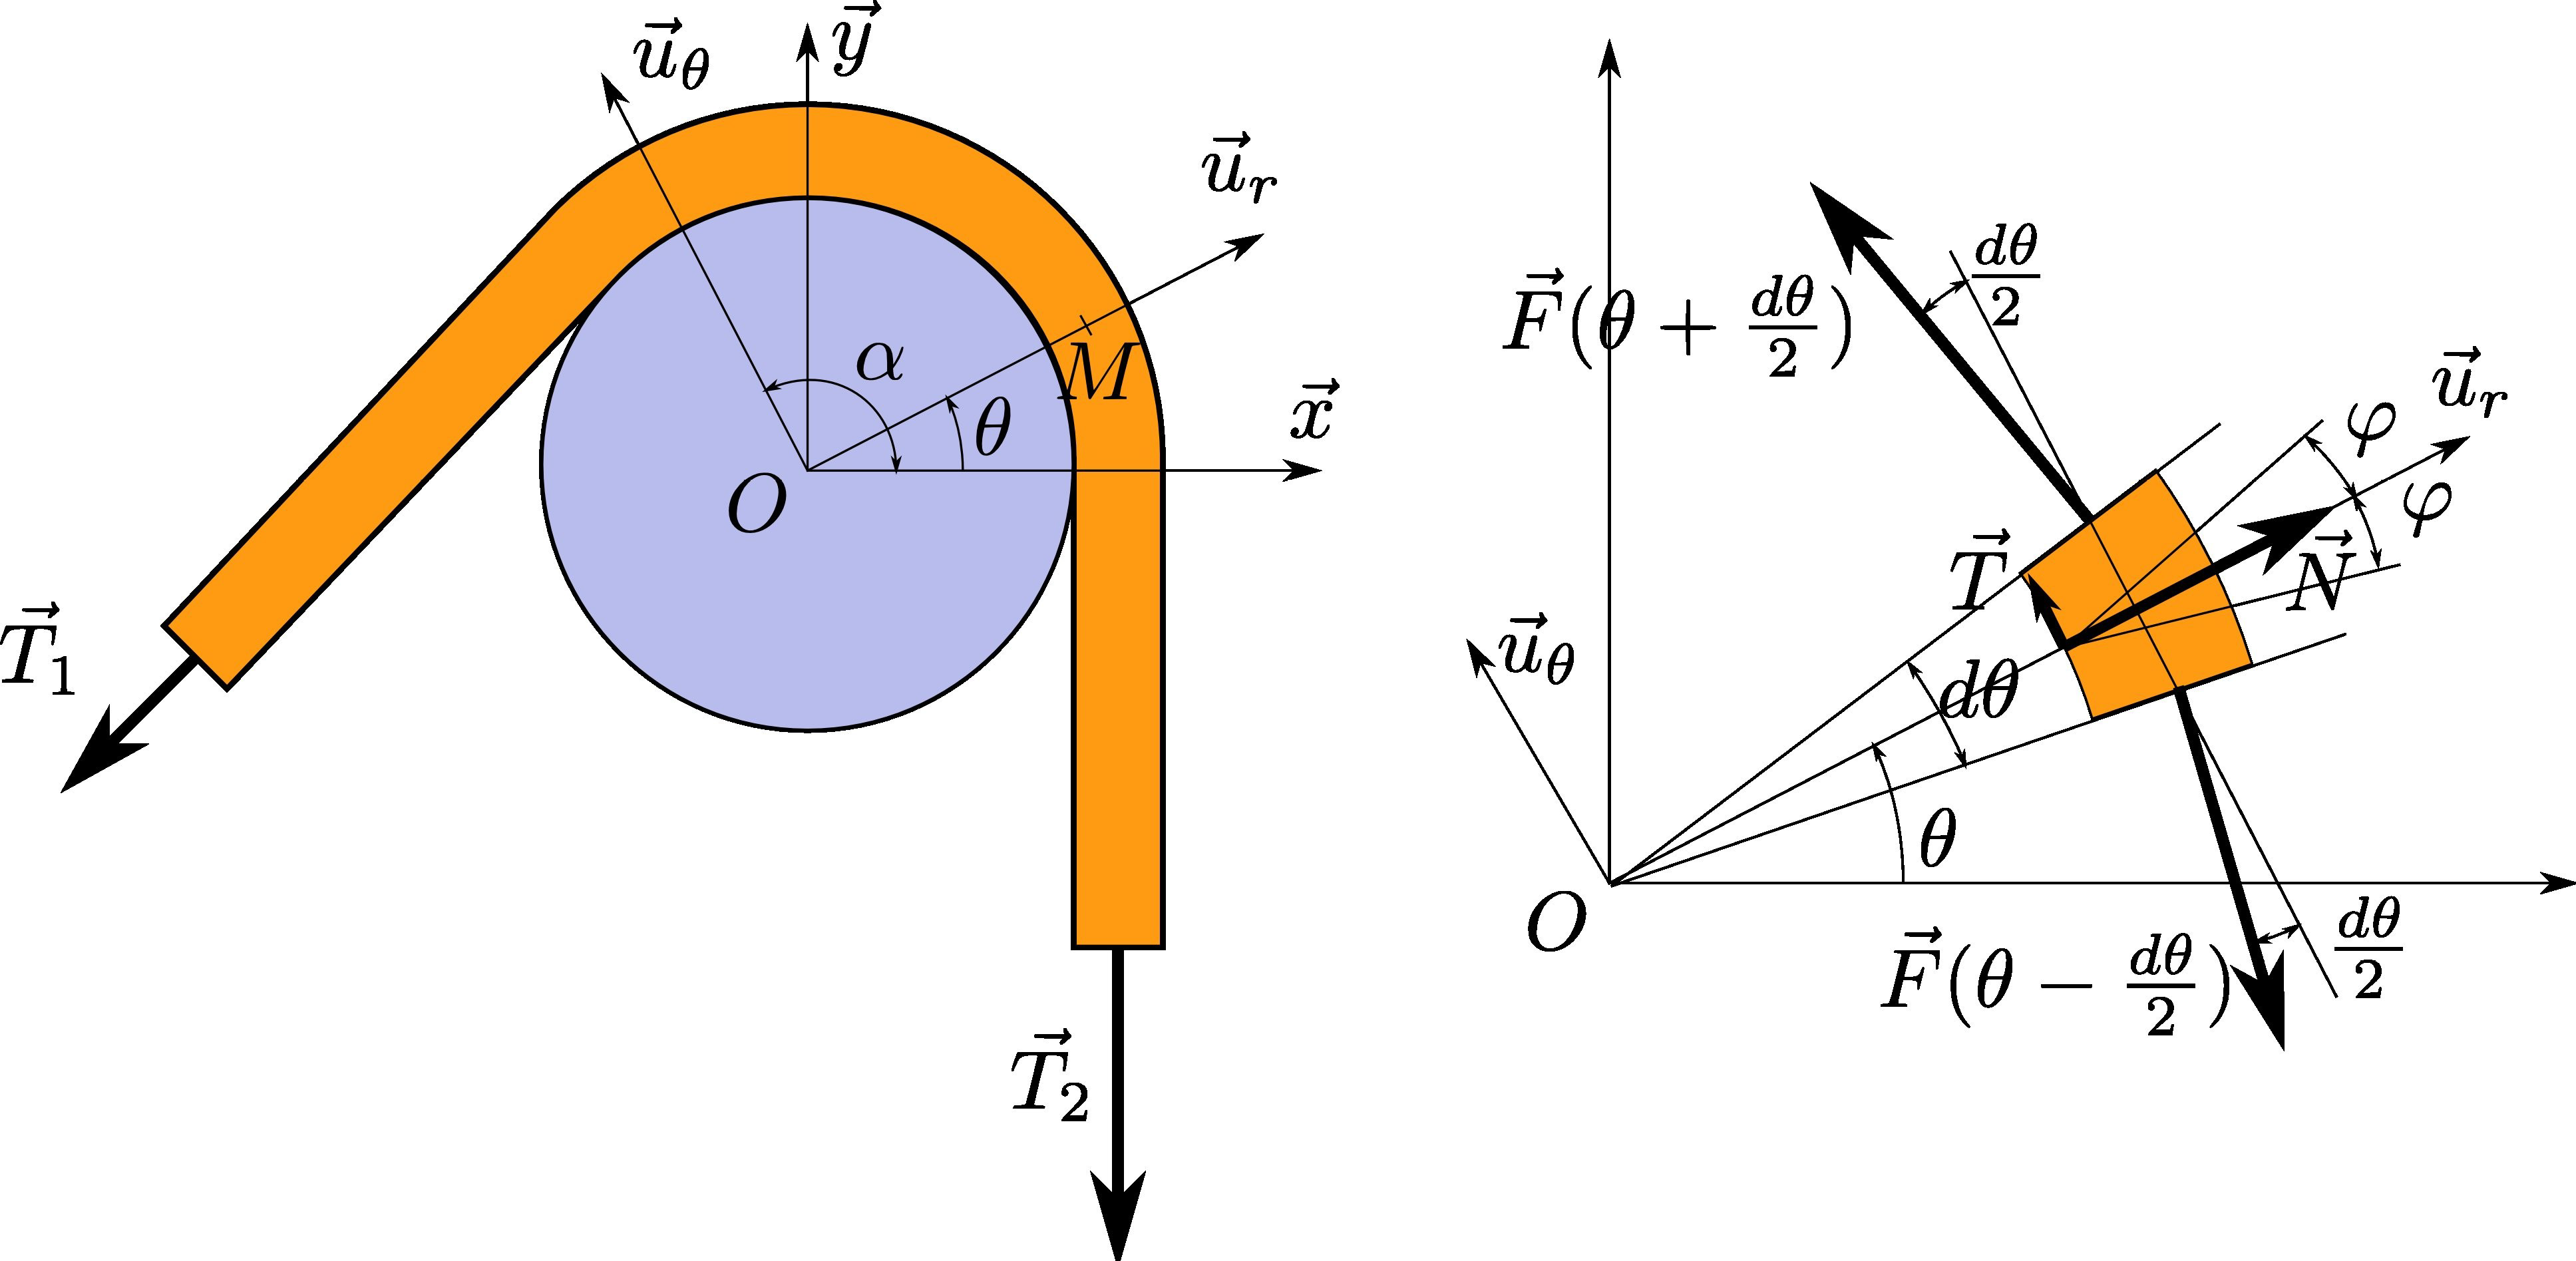
\includegraphics[width=\linewidth]{fig_01.png}
\caption{Sous-système SEIS \label{fig_01}}
\end{marginfigure}


On s'intéresse ici au système de déploiement du sous-système SEIS. Il est basé sur un instrument hybride composé :
\begin{itemize}
\item d'un système de déploiement (DPL);
\item d'une sphère (SEIS) comportant trois capteurs sismiques à très larges bandes et leurs capteurs de
température;
\item d'une boîte électronique d'acquisition dont la structure est donnée par le diagramme de
définition des blocs. 
\end{itemize}

On donne figure \ref{fig_06} le diagramme partiel des exigences.


La figure \ref{fig_07} représente la structure du système de déploiement DPL.

\begin{figure}[!h]
\centering
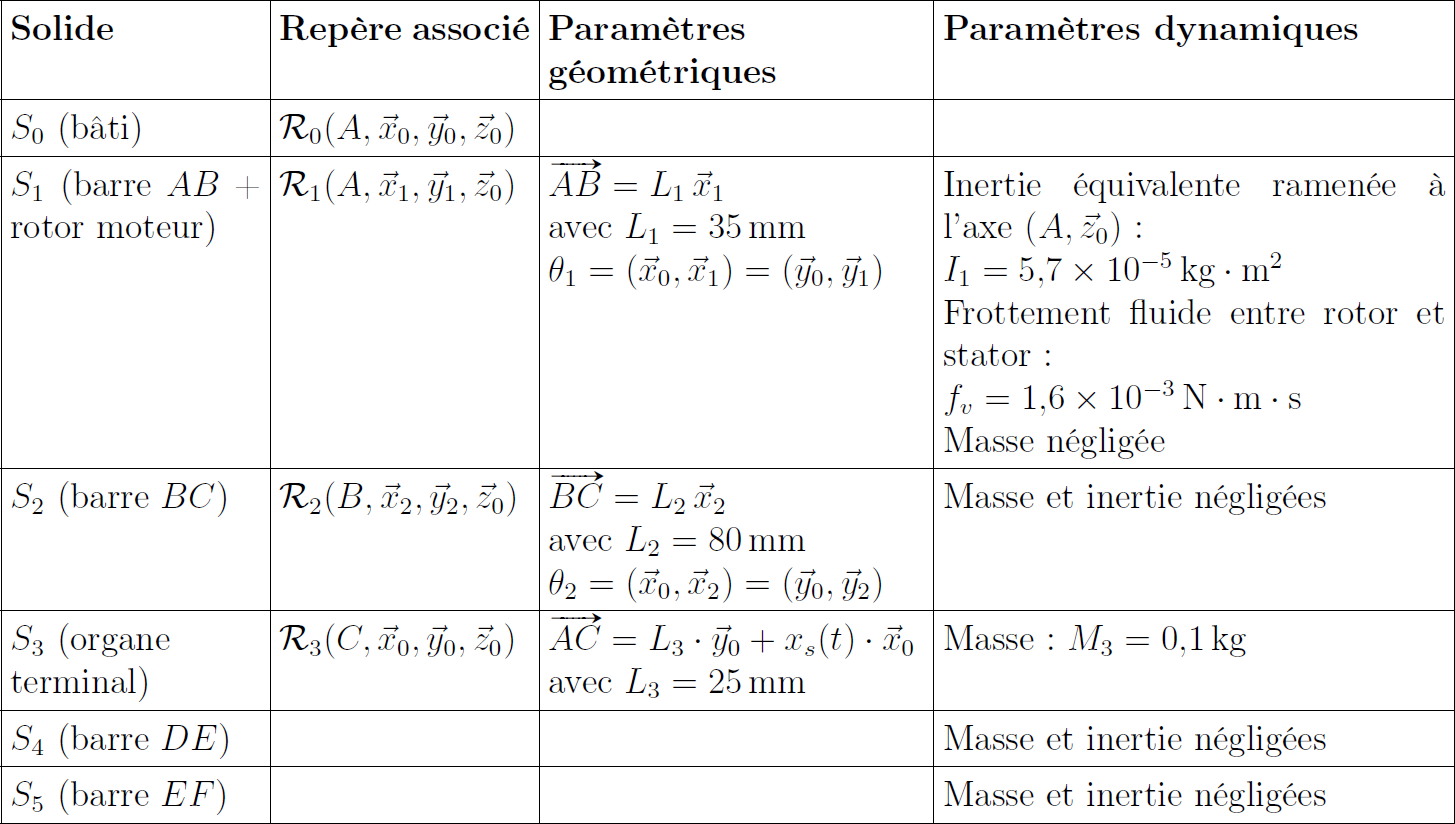
\includegraphics[width=\linewidth]{fig_07.png}
\caption{Schématisation cinématique du bras de déploiement \label{fig_07}}
\end{figure}




\paragraph*{Bâti 0}
Le bâti 0 est doté du repère $\rep{0} \repere{O}{x_0}{y_0}{z_0}$.

\paragraph*{Bras 1}

Le bras 1 est doté du repère $\rep{1} \repere{O}{x_1}{y_1}{z_1}$. Le mouvement de 1 par rapport à 0 est une rotation d'axe $\axe{O}{z_0}$  et d'angle $\theta_1 = \angl{x_0}{x_1}= \angl{y_0}{y_1}$. Le centre d'inertie $G_1$ est paramétré par $\vect{OG_1} = \dfrac{L}{2} \vx{1}$. De plus $\vect{OQ} = L\vx{1}$. Enfin, $m_1 = \SI{352}{g}$ et $L=\SI{0,5}{m}$.


\begin{marginfigure}
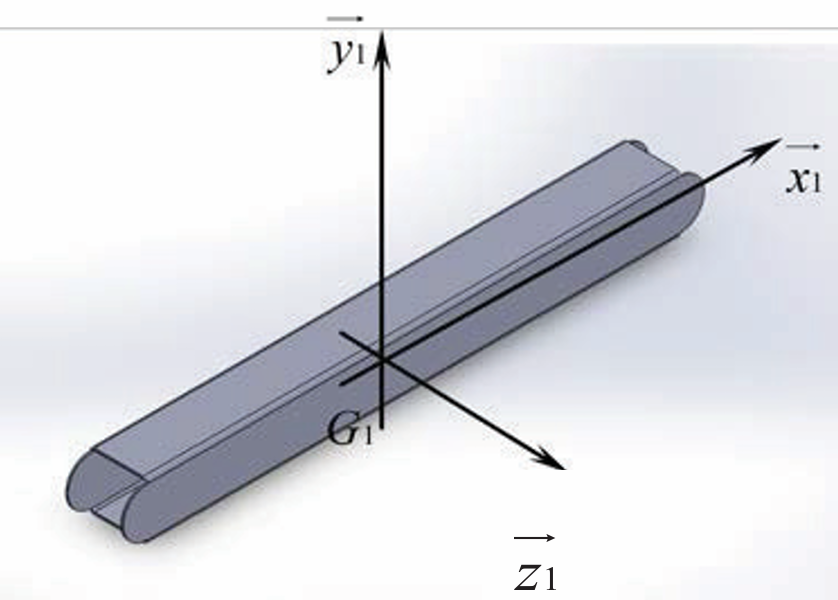
\includegraphics[width=\linewidth]{fig_08.png}
\caption{Bras 1 \label{fig_08}}
\end{marginfigure}

La figure \ref{fig_08} présente le modèle volumique du bras 1. Les plans $\left(G_1,\vx{1},\vy{1}\right)$  et $\left(G_1,\vy{1},\vz{1}\right)$ sont des plans de symétrie matérielle du bras 1.


Le mouvement de 1 par rapport à 0 est commandé par un actionneur $\indice{M}{01}$, constitué d’un moteur pas à pas et d’un réducteur de vitesse à couronne dentée flexible de rapport de transmission $\lambda = 82$, d’encombrement et de masse très faibles en regard des autres solides, logés à l’intérieur de la liaison (0/1).


\paragraph*{Avant-bras 2}
L'avant-bras 2 est doté du repère $\rep{2} \repere{Q}{x_2}{y_2}{z_2}$. Le mouvement de 2 par rapport à 0 est une rotation d'axe $\axe{Q}{z_1}$  et d'angle $\theta_2 = \angl{x_1}{x_2}= \angl{y_1}{y_2}$. Le centre d'inertie $G_2$ est paramétré par $\vect{OG_2} = \dfrac{L}{2} \vx{2}$. De plus $\vect{QP} = L\vx{2}$. Enfin, $m_2 = \SI{352}{g}$ et $L=\SI{0,5}{m}$.

L’extrémité en $P$ est équipée d’une pince de masse négligeable qui saisit la sphère SEIS. On note $\indice{K}{O2}$ le moment d'inertie de l'avant-bras 2 par rapport à l’axe $\axe{O}{z_0}$ dans la position la plus défavorable.  Le mouvement de 2 par rapport à 1 est commandé par un actionneur $\indice{M}{12}$, constitué d’un moteur pas à pas et d’un réducteur de vitesse à couronne dentée flexible de rapport de transmission $\lambda = 82$, d’encombrement et de masse très faibles en regard des autres solides, logés à l’intérieur de la liaison (1/2).


\paragraph*{Sphère du SEIS : S}
On considère que l’amplitude du mouvement (S/2) est très faible. La position (S/0) repérée par : $\vect{OP}= X_P(t) \vx{0} + Y_P(t) \vy{0} $. La masse $m_s = \SI{1,2}{kg}$ est considérée comme ponctuelle en son centre d’inertie $G_S$  par rapport aux autres mouvements. $G_S$  est tel que $\vect{PG_S} = -R \vy{0}$ ($R$ est une constante positive).

On note $\indice{K}{OS}$ le moment d'inertie de la sphère $S$ par rapport à l’axe $\axe{O}{z_0}$  dans la position $\theta_1 =\theta_2 = 0$.


\begin{figure}[!h]
\centering
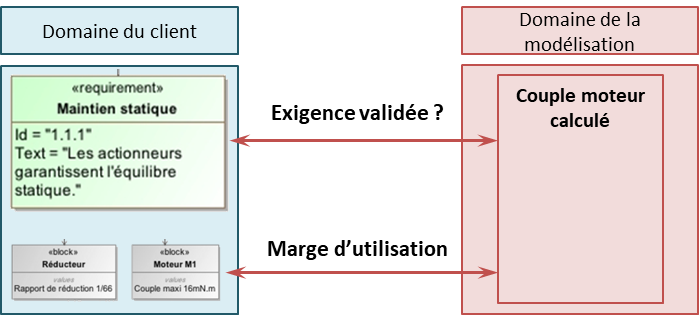
\includegraphics[width=\linewidth]{fig_06.png}
\caption{Diagramme partiel des exigences \label{fig_06}}
\end{figure}


\vfill
